\chapter{Theory \& Methodology}

\section{Theory}

\subsection{Time Series to Image Transformation Methods}

It is necessary to transform Time seires into image representations if we use image based models. Various transformation methods have been proposed to encode time series data into two-dimensional images while preserving temporal dependencies and structural patterns. Among these, we consider Gramian Angular Fields (GAFs), Markov Transition Fields (MTF), and Spectrograms.

\subsubsection*{Gramian Angular Fields (GAFs)}

Gramian Angular Fields represent time series data in a polar coordinate system before encoding it into a square matrix. The key idea behind GAF is to utilize trigonometric functions to capture relationships between different time points, ensuring that temporal dependencies are embedded in the transformed representation. This encoding has been shown to be effective in converting temporal data into images that can be used by deep learning models for tasks such as classification and anomaly detection \parencite{wang2015encoding}. The GAF transformation consists of two main steps:

\begin{enumerate}
    \item \textbf{Normalization and Angular Encoding}: Convert the time series into an angular representation.
    \item \textbf{Gramian Matrix Construction}: Compute either summation-based or difference-based transformations to form a 2D matrix.
\end{enumerate}

 Given a time series $ X = \{ x_{1}, x_{2}, ... , x_{N} \} $  where $x$ represents the signal amplitude at different time points, we first normalize the values to be within $[-1,1]$ sing min-max normalization:
\begin{equation}
    \tilde{x_{i}} = \frac{2(x_{i} - min(X))}{max(X) - min(X)} -1
\end{equation}

Next, we map these normalized values into angular space using the inverse cosine function:
\begin{equation}
    \theta_{i} = \arccos(\tilde{x_{i}})
\end{equation}

This transformation ensures that the entire time series is represented as angles in a polar coordinate system. \\

Once the time series is represented in angular form, the Gramian matrix is computed based on the trigonometric sum or difference of angles between time points. There are two primary types of GAF representations. \\

\textbf{Gramian Angular Summation Field (GASF)} \\

GASF captures the magnitude and global trend of the time series by computing the cosine summation of angular values:
\begin{equation}
    GASF(i,j) = cos( \theta_{i} + \theta_{j})
\end{equation}

GASF preserves the overall shape and pattern of the time series, making it useful for applications where global structures are important. \\

\textbf{Gramian Angular Difference Field (GADF)} \\

GADF highlights fluctuations and dynamic changes in the time series by computing the sine difference of angular values:
\begin{equation}
    GADF(i,j) = sin( \theta_{i} - \theta_{j})
\end{equation}

GADF focuses on transitions and local variations, making it useful for tasks where short-term changes are significant.

\subsubsection*{Markov Transition Fields (MTF)}

Markov Transition Fields (MTFs) represent the probability of transitioning between different states within a time series. This method is based on the principles of Markov Chains, where the probability of moving to a future state depends solely on the current state. MTFs effectively preserve both global and local temporal structures by encoding state transitions over time into a 2D image-like representation \parencite{wang2015imaging}. The MTF transformation consists of the following key steps: 

\begin{enumerate}
    \item \textbf{Discretization of the Time Series}: Convert continuous values into discrete states.
    \item \textbf{Computation of the Markov Transition Matrix}: Determine transition probabilities between states.
    \item \textbf{Construction of the Markov Transition Field}: Encode state transitions into a structured 2D representation.
\end{enumerate}

Given a time series $ X = \{ x_{1}, x_{2}, ... , x_{N} \} $ we first normalize and discretize the values into $Q$ quantile bins to create a finite number of states. Discretization allows us to model transitions as a probabilistic system:
\begin{equation}
    Q(X) = \{ q_{1}, q_{2}, ... , q_{N} \}, \qquad q_{i}\in \{ 1, 2, ... , Q \}
\end{equation}
where each $q$ represents the state of the time series at a given time step after quantization. \\

Once the time series is discretized, we compute the Markov Transition Matrix (MTM), which captures the probabilities of transitioning from one state to another. The probability of moving from state $q_{i}$ to state $q_{j}$ is calculated as:
\begin{equation}
    P(q_{i} \mid q_{j}) = \frac{\text{Number of transitions from } q_{i} \text{ to } q_{j}}{\text{Total number of transitions from } q_{i}}
\end{equation}

The MTM provides a compact summary of state transitions and characterizes the underlying structure of the time series. \\

The Markov Transition Field (MTF) extends the MTM into a two-dimensional matrix by encoding the transition probabilities between all time points. This is done by assigning the transition probability from $q_i$ to $q_j$ at different time steps:
\begin{equation}
    MTF(i,j) = P( q_j \mid q_i)
\end{equation}

This results in a N × N matrix, where each element represents the probability of transitioning between states at different timestamps. The MTF matrix retains both local and global transition structures, preserving the temporal dependencies inherent in the time series.

\subsubsection*{Spectrograms}

A spectrogram is a visual representation of the frequency content of a signal as it varies with time. It is commonly used in time-frequency analysis to explore how the spectral characteristics of a signal evolve, especially in non-stationary signals such as audio, biomedical, and EEG data \parencite{welch2003use}. The most widely used method for computing spectrograms is the Short-Time Fourier Transform (STFT). \\

The STFT segments a signal into overlapping time windows and computes the Fourier Transform within each window to obtain a time-localized frequency spectrum. Mathematically, the STFT of a signal $x(t)$ is defined as:
\begin{equation}
    \text{STFT }(\tau, f) = \int_{-\infty}^{\infty} x(t)w(t-\tau)e^{-j2\pi ft} \,dx 
\end{equation}
where:
\begin{itemize}
    \item $x(t)$ is the time-domain signal,
    \item $w(t)$ is a window function (e.g., Hamming, Hanning, or Gaussian),
    \item $\tau$ represents time,
    \item $f$ represents frequency.
\end{itemize}

The spectrogram is then obtained as the squared magnitude of the STFT:
\begin{equation}
    \text{Spectrogram }(\tau, f) =  \lvert \text{ STFT }(\tau , f) \rvert ^{2}
\end{equation}

 This results in a time-frequency representation where each pixel in the spectrogram represents the power of a particular frequency at a given time.


\subsection{Frequency Downsampling Methods}

Frequency downsampling is a crucial preprocessing step in time series analysis. It involves reducing the frequency resolution while retaining essential spectral information, allowing efficient data processing and reducing computational complexity. Two widely used techniques for frequency downsampling are the Fast Fourier Transform (FFT) and the Discrete Wavelet Transform (DWT). \\

\subsubsection*{Fast Fourier Transform (FFT)}

The Fast Fourier Transform (FFT) is an efficient algorithm for computing the Discrete Fourier Transform (DFT), which decomposes a signal into its constituent frequency components. It is widely used in signal processing for spectral analysis, filtering, and feature extraction. The FFT significantly reduces the computational burden of DFT calculations, making it feasible to analyze large-scale time series data \parencite{oppenheim1999discrete}. \\

The Discrete Fourier Transform (DFT) of a discrete time-domain signal $x(n)$ of length $N$ is defined as:
\begin{equation}
    X(k) = \sum_{n=0}^{N-1} x(n)e^{-j2\pi kn/N}, \qquad k = 0,1, ..., N-1
\end{equation}
where:
\begin{itemize}
    \item $X(k)$ represents the Fourier coefficients corresponding to different frequency components,
    \item $e^{-j2\pi kn/N}$ is the complex exponential basis function.
\end{itemize}
 
Computing this equation directly requires $O(N^2)$ operations, making it inefficient for large $N$. The FFT algorithm optimizes this computation, reducing the complexity to $O(N \log N)$ , thereby making it significantly faster \parencite{cooley1965algorithm}. \\

The FFT employs a divide-and-conquer approach, recursively breaking down a large Discrete Fourier Transform (DFT) problem into smaller DFT computations. The most widely used version, the Cooley-Tukey algorithm, leverages the periodicity and symmetry of Fourier basis functions to reduce redundant calculations. The FFT process begins by dividing the original sequence into even-indexed and odd-indexed components, followed by recursively computing the DFT for each smaller sequence. Finally, the results are efficiently combined using butterfly operations to obtain the final transform. For a signal of length $N$, the FFT is most efficient when $N$ is a power of 2, although alternative methods exist for handling arbitrary-length signals. \\

FFT is commonly used for \textbf{frequency downsampling}, which involves reducing the sampling rate while preserving essential frequency content. The process includes:
\begin{enumerate}
    \item \textbf{Apply FFT} to convert the time-domain signal to the frequency domain.
    \item \textbf{Remove high-frequency components} beyond the desired Nyquist frequency.
    \item \textbf{Apply Inverse FFT (IFFT)} to reconstruct the downsampled signal.
\end{enumerate}
This technique is useful for eliminating high-frequency noise and retaining low-frequency EEG features essential for sleep stage classification.

\subsubsection*{Discrete Wavelet Transform (DWT)}

The Discrete Wavelet Transform (DWT) is a widely used signal processing technique that decomposes a signal into different frequency components while preserving temporal information. Unlike the Fourier Transform, which represents a signal purely in the frequency domain, DWT provides a time-frequency representation, making it particularly useful for analyzing non-stationary signals \parencite{mallat1999wavelet}. \\

Given a discrete signal $x[n]$, the DWT performs convolution with a low-pass filter $h[n]$  (scaling function) and a high-pass filter $g[n]$  (wavelet function):
\begin{itemize}
    \item Approximation coefficients (Low-frequency components):
    \begin{equation}
        A[n] = (x * h)[2n] = \sum_k x[k]h[2n-k]
    \end{equation}
    \item Detail coefficients (High-frequency components):
    \begin{equation}
        D[n] = (x * g)[2n] = \sum_k x[k]g[2n-k]
    \end{equation}
\end{itemize}
Here, $A[n]$ represents the low-frequency sub-band, which captures the coarse structure of the signal, while $D[n]$ represents the high-frequency sub-band, capturing the detailed variations. After filtering, downsampling by 2 is applied, which means keeping every second sample:
\begin{equation}
    A_d [n] = A[n] \qquad \text{(Low-frequency downsampling)}
\end{equation}
\begin{equation}
    D_d [n] = D[n] \qquad \text{(High-frequency downsampling)}
\end{equation}
This step effectively reduces the signal resolution by a factor of 2 in both the approximate (low-frequency) and detail (high-frequency) coefficients. Applying DWT recursively to the approximation coefficients $A_d [n]$, we obtain multiple levels of decomposition. Each level further reduces the frequency resolution while maintaining the time-domain localization \parencite{subasi2007eeg}.

\subsection{Deep Convolutional Generative Adversarial Networks (DCGANs)}
 
Deep Convolutional Generative Adversarial Networks (DCGANs) are a variant of Generative Adversarial Networks (GANs) that leverage deep convolutional neural networks for both the generator and discriminator. This architecture is particularly adept at generating synthetic images, which can be crucial in scenarios where real images are scarce or difficult to obtain. In this section, we delve into the theoretical underpinnings of DCGANs, focusing on their architecture, mathematical formulations, and the adversarial process that drives their ability to generate realistic images \parencite{radford2015unsupervised}. \\

A DCGAN consists of two primary components: a generator and a discriminator. The generator takes a random noise vector as input and produces a synthetic image, while the discriminator evaluates the input image (real or synthetic) and outputs a probability indicating whether the image is real or fake. Figure \ref{fig:dcgan} illustrates the architecture of DCGAN.\\
\begin{figure}[H]
    \centering
    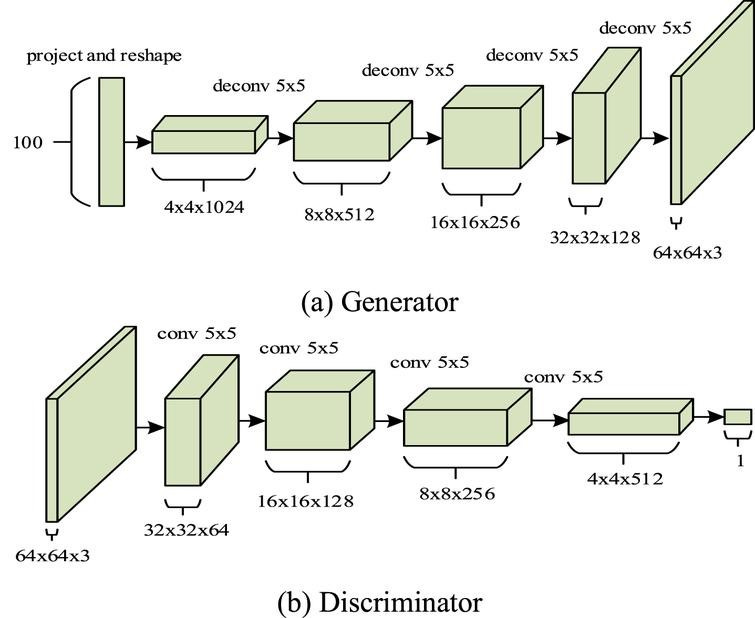
\includegraphics[width=0.7\linewidth]{Figures/dcgan.png}
    \caption{Architecture of DCGAN}
    \label{fig:dcgan}
\end{figure} 

\subsubsection*{Generator}

The generator in a DCGAN is a deep convolutional neural network designed to map a random noise vector $z \sim p_z(z) $  to a high-dimensional image space. This process can be formulated as:
\begin{equation}
    G : z \rightarrow x_{\text{fake}}
\end{equation}
where $ G(z; \theta _G) $ represents the generator network parameterized by $ \theta_G $. The network consists of a series of transposed convolutional (or deconvolutional) layers, batch normalization, and ReLU activations, except for the final layer, which often uses a Tanh activation to produce pixel values in the range $ [-1,1]$ . Mathematically, the generator optimizes the following objective function:
\begin{equation}
    \min_{\theta_G} \mathbb{E}_{z \sim p_z (z)}[log(1-D(G(z)))]
\end{equation}
where $D(G(z))$ is the probability assigned by the discriminator to the generated image being real.

\subsubsection*{Discriminator}

The discriminator is a deep convolutional neural network designed to classify whether a given image is real or synthetic. It takes an image $x$ as input and outputs a probability $ D(x) $  indicating the likelihood that the image is real. Formally, the discriminator is represented as:
\begin{equation}
    D : x \rightarrow [0,1]
\end{equation}
where $ D(x: \theta_D) $ is the discriminator network parameterized by $ \theta_D$ . The architecture consists of a series of convolutional layers with LeakyReLU activations and batch normalization, ending in a sigmoid activation function to produce a probability score. The discriminator is trained to maximize the likelihood of correctly classifying real and fake images, optimizing the following loss function:
\begin{equation}
    \max_{\theta_D} \mathbb{E}_{x \sim p_{\text{data}}(x)}[log D(x)] + \mathbb{E}_{z \sim p_z (z)}[log (1-D(G(z)))]
\end{equation}

\subsubsection*{Adversarial Training Process}

DCGAN training follows the standard GAN framework, where the generator and discriminator are trained in an adversarial manner. The overall objective function of the GAN is given by:
\begin{equation}
    \min_G \max_D V(G,D) = \mathbb{E}_{x \sim p_{\text{data}}(x)}[log D(x)] + \mathbb{E}_{z \sim p_z (z)}[log (1-D(G(z)))]
\end{equation}
This formulation defines a two-player minimax game, where the generator seeks to minimize the discriminator’s ability to distinguish real from fake images, while the discriminator seeks to maximize its classification accuracy. The training is performed iteratively, alternating between updating $ \theta_D$ and $ \theta_G $ , typically using stochastic gradient descent (SGD) or Adam optimization.

\subsection{Vision Transformers (ViTs)}

Vision Transformers (ViTs) are a novel approach to image processing that replaces traditional convolutional neural networks (CNNs) with self-attention mechanisms, initially developed for natural language processing (NLP). Unlike CNNs, which rely on hierarchical feature extraction, ViTs process images as sequences of smaller patches, allowing them to capture long-range dependencies more effectively. This section explores the architecture and working of Vision Transformers, detailing their key components and mathematical formulations \parencite{dosovitskiy2020image}. Figure \ref{fig:vit} illustrates the ViT architecture.
\begin{figure}[H]
    \centering
    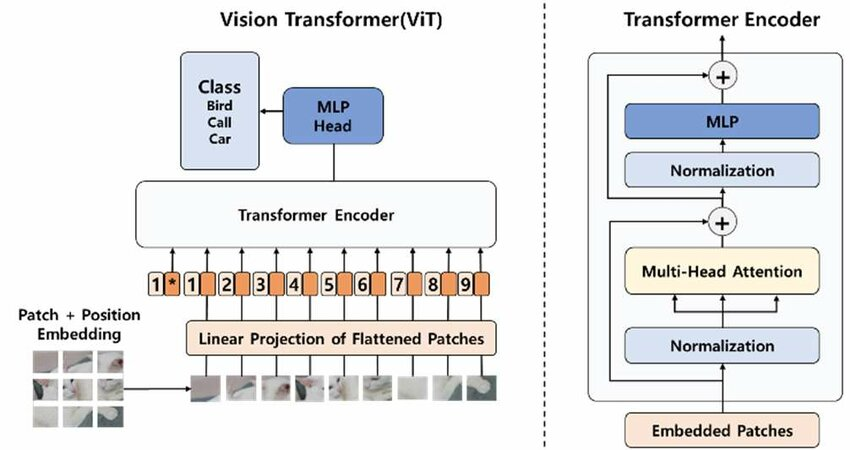
\includegraphics[width=0.7\linewidth]{Figures/vit.png}
    \caption{Architecture of ViT}
    \label{fig:vit}
\end{figure} 

\subsubsection*{Image Patch Embedding}

In ViTs, an image $ X \in  \mathbb{R}^{H \times W \times C}$ (where $H$ and $W$ are the height and width, and $C$ is the number of channels) is divided into a grid of non-overlapping patches, each of size $ P \times P$ . The number of patches, $N$ , is given by:
\begin{equation}
    N = \frac{H \times W}{P^2}
\end{equation}
Each patch is then flattened into a vector $ x_p \in \mathbb{R}^{P^2 C}$, and a trainable linear projection $E$ maps it to a lower-dimensional embedding space of size $D$. 
\begin{equation}
    z_p = Ex_p \in \mathbb{R}^D
\end{equation}
Additionally, a learnable class token $z_0$ is appended to the sequence, similar to the [CLS] token in NLP Transformers. The final input sequence $Z$ is:
\begin{equation}
    Z = [z_0 ; z_1 ; ... ; z_N] \in \mathbb{R}^{(N+1)\times D}
\end{equation}

\subsubsection*{Positional Encoding}

Since Transformers do not inherently capture spatial information, positional encodings are added to the patch embeddings. These are computed using sine and cosine functions:
\begin{equation}
    PE_{(pos,2i)} = sin \left( \frac{pos}{10000^{2i/D}} \right)
\end{equation}
\begin{equation}
    PE_{(pos,2i+1)} = cos \left( \frac{pos}{10000^{2i/D}} \right)
\end{equation}
where $pos$ is the position index, and $i$ is the embedding dimension index. These encodings are added to the patch embeddings:
\begin{equation}
    Z = Z + PE
\end{equation}

\subsubsection*{Multi-Head Self-Attention (MHSA)}

A core component of ViTs is the self-attention mechanism, which allows each token (patch) to attend to all others. Given an input sequence $Z$, three weight matrices $W_Q$ , $W_K$ , $W_V$ and  project it into query, key, and value representations:
\begin{equation}
    Q = ZW_Q \qquad K = ZW_K \qquad V = ZW_V
\end{equation}
The scaled dot-product attention is then computed as:
\begin{equation}
    Attention(Q,K,V) = softmax \left( \frac{QK^T}{\sqrt{D_k}} \right)V
\end{equation}
where $D_k$ is the dimension of the key vectors. Multi-head self-attention (MHSA) applies this mechanism in parallel using multiple heads:
\begin{equation}
    MHSA(Z) = Concat(head_1, head_2, ... , head_k)W_o
\end{equation}
where each head is computed as:
\begin{equation}
    head_i = Attention(Q_i, K_i, V_i)
\end{equation}

\subsubsection*{Feedforward Network (FFN)}

Following MHSA, each token representation passes through a Feedforward Network (FFN), consisting of two linear layers with a GELU activation function:
\begin{equation}
    FFN(x) = W_2 \cdot GELU(W_1 x+ b_1) + b_2
\end{equation}
To stabilize training, layer normalization is applied before MHSA and FFN, and residual connections are added:
\begin{equation}
    Z^{'} = Z + MHSA(LayerNorm(Z))Z^{''} = Z^{'} + FFN(LayerNorm(Z^{'}))
\end{equation}
The final output sequence $Z^{''}$  contains a special class token $z_0$, which serves as the global representation of the image. A linear classifier maps it to the final class predictions:
\begin{equation}
    \hat{y} = W_c z_0 + b_c
\end{equation}
where $W_C$ and $b_c$ are the weights and bias of the classification layer.

\section{Methodology}

\subsection{Signal Pre-processing}

Raw PSG signals often contain unwanted noise from various sources, including environmental interference, power line noise, motion artifacts, and physiological noise. To enhance signal quality, we applied a combination of low-pass filtering, high-pass filtering, and notch filtering to remove unwanted frequency components while preserving relevant information. High-Pass Filtering Used to remove slow drifts and DC components from the signals. Low-Pass Filtering applied to remove high-frequency noise and muscle artifacts.
Notch Filtering used to eliminate power line interference. Table \ref{tab:signal_specs} summarizes the specific filtering parameters used for different signal channels.

\begin{table}[H]
    \centering
    \renewcommand{\arraystretch}{0.7}
    \begin{tabular}{|c|c|c|c|c|c|}
        \hline
        \multirow{2}{*}{\textbf{Signal Type}} & \multicolumn{2}{c|}{\textbf{Value Range}} & \multicolumn{3}{c|}{\textbf{Filter Frequency}} \\
        \cline{2-6}
        & \textbf{Minimum} & \textbf{Maximum} & \textbf{High-pass} & \textbf{Low-pass} & \textbf{Notch} \\
        \hline
        EEG & -35 µV & 35 µV & 0.5 Hz & 35 Hz & 60 Hz \\
        \hline
        EOG & -35 µV & 35 µV & 0.3 Hz & 35 Hz & 60 Hz \\
        \hline
        ECG & -0.5 mV & 0.5 mV & 0.3 Hz & 70 Hz & 60 Hz \\
        \hline
        EMG & -35 µV & 35 µV & 10 Hz & 70 Hz & 60 Hz \\
        \hline
        
    \end{tabular}
    \caption{Signal specifications and filtering parameters}
    \label{tab:signal_specs}
\end{table}

\subsection{Experiment 1: Performance Evaluation of Different Image Transformation Techniques}

This experiment investigates the effectiveness of various image transformation techniques for representing PSG signals in sleep stage classification using Vision Transformers (ViTs). The transformation methods evaluated include Spectrograms, Gramian Angular Difference Field (GADF), Gramian Angular Summation Field (GASF), and Markov Transition Field (MTF). The primary objective is to determine which transformation method provides the most informative representation for Vision Transformer-based classification. \\

16 PSG channels (F7-T3, T3-T5, Fp1-F3, F3-C3, C3-P3, P3-O1, Fp2-F4, F4-C4, C4-P4, P4-O2, F8-T4, T4-T6, EOG, EMG, ECG, and Avg) were selected for this study and segmented into 30-second epochs. Each channel within an epoch was transformed into an image using the designated method. The resulting images were subsequently concatenated into a 4×4 matrix, forming a single image representation per epoch, as illustrated in Figure \ref{fig:psg_channel_img}. \\ 

A total of 12,000 epochs (with 2,000 epochs per sleep stage) were selected from the All Subjects Dataset (DS9). The pre-trained Vision Transformer (ViT-B/16) model was then fine-tuned to ensure a fair comparison across different transformation techniques.

\begin{figure}[H]
    \centering
    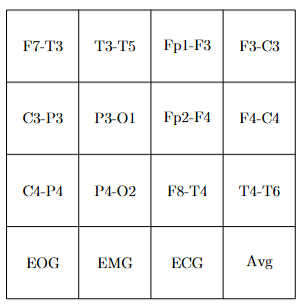
\includegraphics[width=0.5\linewidth]{Figures/psg_channels.png}
    \caption{16 PSG channels to form a unified image representation.}
    \label{fig:psg_channel_img}
\end{figure} -

\subsection{Experiment 2: Effect of Sampling Frequency and Resampling Method}

This experiment investigates the impact of different sampling frequencies and resampling methods on sleep stage classification performance. In this, 4 sampling frequencies were evaluated: 512 Hz (original), 256 Hz, 128 Hz, and 64 Hz. Additionally, two resampling methods, Fast Fourier Transform (FFT) and Discrete Wavelet Transform (DWT) were applied to determine the most effective approach. \\

Following the same approach as in Experiment 1, a total of 12,000 epochs (2,000 per sleep stage) were selected from the All Subjects Dataset (DS9). These epochs were then down-sampled to 256 Hz, 128 Hz, and 64 Hz using Fast Fourier Transform (FFT) and Discrete Wavelet Transform (DWT). The images were generated using the transformation method identified as the most effective in Experiment 1. Finally, the pre-trained Vision Transformer (ViT-B/16) model was fine-tuned to ensure a fair comparison across the different sampling frequencies and resampling methods. \\

\subsection{Experiment 3: Effectiveness of Pre-Trained vs. From-Scratch Vision Transformers}

This experiment aims to compare the performance of trained from scratch ViT models with pre-trained ViT models for sleep stage classification. Both balanced and imbalanced datasets are utilized in this experiment. \\

For this experiment, the All Subjects Dataset (DS9) was used again. Images were generated using the best methods identify in Experiments 1 and 2. The data was then used to evaluate both imbalanced and balanced datasets. To address the class imbalance, up-sampling was applied to create a balanced dataset. Once both balanced and imbalanced datasets were prepared, the ViT model was first trained from scratch and tuned to achieve the best performance. Subsequently, the pre-trained ViT-B/16 model was fine-tuned for both datasets.

\subsection{Experiment 4: Effectiveness of Different Pre-Trained Vision Transformers}

Given that fine-tuning the ViT-B/16 model outperformed training from scratch, further experiments have to conduct to compare the performance of various pre-trained ViT models. The aim was to identify the model that provides the best classification accuracy while ensuring optimal computational efficiency. \\

Based on the results from Experiments 1 and 2, a balanced image dataset was created using the DS9 dataset. The following pre-trained ViT models were then fine-tuned on this dataset: ViT-B/32, DeiT-B, Swin-B, BEiT-B, and PVT-Small.

\subsection{Experiment 5: Training and Tuning DCGAN for Synthetic Image Generation}

To address the challenges of subject-to-subject variability and class imbalances in sleep stage classification, GAN-based data augmentation was employed. The primary objective was to enhance the diversity of training samples, thereby improving model generalization. Specifically, a Deep Convolutional Generative Adversarial Network (DCGAN) was implemented to generate realistic synthetic data, contributing to a more balanced and representative training set. \\

First, images for the DS9 dataset were generated based on the results from Experiments 1 and 2. The dataset was then split into 70\% for training and 30\% for validation. Subsequently, various architectures DCGANs were trained and tuned to generate synthetic PSG images.

\subsection{Experiment 6: Effectiveness of GAN-Augmented Data}

In Experiment 5, the primary objective was to train a DCGAN model for the generation of synthetic PSG image representations. The focus of this experiment was to evaluate the effectiveness of the generated synthetic data in improving sleep stage classification performance. \\

First, images for the DS9 dataset are generated based on the results from Experiments 1 and 2. These images are then separated according to the corresponding sleep stages. Next, the trained DCGAN model is fine-tuned for each sleep stage class, generating 20,000 synthetic images per class. \\

Following this, the best-performing classification model identified after Experiment 4 is selected. This model is then fine-tuned on three different datasets:
\begin{enumerate}
    \item The \textbf{original dataset} (with upsampling applied only in this case)
    \item The \textbf{GAN-augmented dataset} (containing only synthetic images)
    \item A \textbf{mixed dataset} (comprising both original and synthetic images)
\end{enumerate}
For each dataset, 10,000 images per class randomly used for training.

\subsection{Final Model Selection}

Following Experiment 6, the best-performing model is identified as the optimal model for this study. After selecting this model, its performance is further evaluated on DS1–DS8 datasets to assess its generalization capability across different data distributions.\\

\begin{figure}[H]
    \centering
    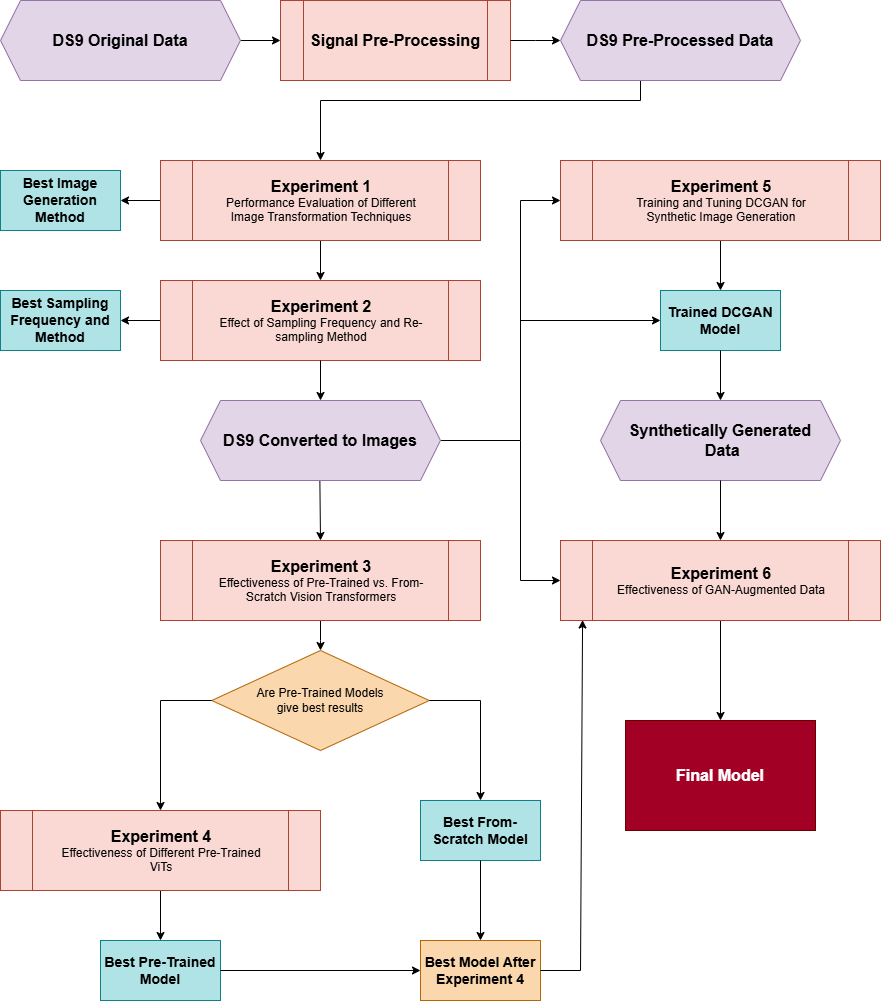
\includegraphics[width=1\linewidth]{Figures/methodology.png}
    \caption{Overview of Methodology}
    \label{fig:methodology_overview}
\end{figure} 
